\documentclass[main.tex]{subfiles}

\begin{document}
The graphical user interface has been developed following two guidelines: to be responsive and dynamic.\\
The responsiveness of a GUI means its adaptability to different screen sizes, and in order to achieve this goal, it has been decided to make a strong use of the composite pattern implemented in Supercollider. In fact, each GUI object is a sublass of the generic class View. Each component can contain different components, thus creating a tree-like structure. In the actual implementation each GUI component passes itself to the constructor of the children components, so that they can infer its dimensions and scale their dimensions accordingly.\\
 In the main script, the sizes of the screen are retrieved through a system call, and those quantities are used to scale every other portion of the GUI. Going up to the hierarchy of components and subcomponents we reach the main window that contains the whole application, which is proportional to the screen size. This implementation allows to have a user interface that scales with the screen dimensions.
In order to have a dynamic GUI, that allows the user to create and erase instances of the various instruments, it has been used a factory pattern, which is a common design pattern in object oriented programming. To implement it, it is necessary to make an abstraction on the objects that are created, that in this case are simply instruments (Inst class), and provide a class that is responsible for the creation of such objects (Inst Factory).\\
The class diagram below(\autoref{fig:2}) depicts the simplified architecture for the instruments creation and behaviour. The Supercollider classes are omitted for the sake of clarity.
\begin{figure}[htbp]
\centering
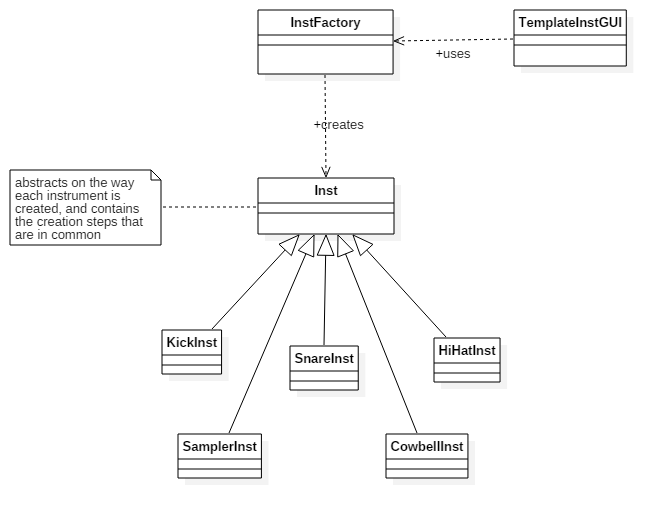
\includegraphics[height=8cm, width=12cm]{images/factory_pattern_uml.png}
\caption{Class diagram of the application}
\label{fig:2}
\end{figure}

\end{document}